% Copyright 2019 the authors. All rights reserved.

% TODO:
% -

\documentclass[twocolumn]{aastex62}

\usepackage[T1]{fontenc}
\usepackage{amsmath}

% typography
\setlength{\parindent}{1.\baselineskip}
\newcommand{\acronym}[1]{{\small{#1}}}
\newcommand{\package}[1]{\textsl{#1}}
\newcommand{\gaia}{\textsl{Gaia}}
\newcommand{\pans}{\textsl{Pan-STARRS}}
\newcommand{\DR}{\acronym{DR2}}
\newcommand{\msun}{\textrm{M}_\odot}
\newcommand{\kpc}{\textrm{kpc}}
\newcommand{\kms}{\ensuremath{\textrm{km}~\textrm{s}^{-1}}}
\newcommand{\bs}[1]{\boldsymbol{#1}}
\newcommand{\masyr}{\ensuremath{\textrm{mas}~\textrm{yr}^{-1}}}
\newcommand{\feh}{\ensuremath{[\textrm{Fe} / \textrm{H}]}}
\newcommand{\given}{\,|\,}

\newcommand{\ab}[1]{{\color{red} AB: #1}}


\newcommand{\sectionname}{Section}
\newcommand{\equationname}{Equation}
\renewcommand{\tablename}{Table}
\usepackage{upgreek}

\newcommand{\todo}[1]{{\color{red} TODO: #1}}

\newcommand{\changes}[1]{{\textbf{#1}}}
% \newcommand{\changes}[1]{{#1}}

% aastex parameters
% \received{not yet; THIS IS A DRAFT}
%\revised{not yet}
%\accepted{not yet}
% % Adds "Submitted to " the arguement.
% \submitjournal{ApJ}
\shorttitle{pal~5's biggest fan}
\shortauthors{bonaca et al.}

%@arxiver{}

\begin{document}\sloppy\sloppypar\raggedbottom\frenchspacing % trust me

\title{Variations in the width, density, and direction of the Palomar~5 tidal tails}

\author[0000-0002-7846-9787]{Ana~Bonaca}
\affiliation{Center for Astrophysics | Harvard \& Smithsonian, Cambridge, MA 02138, USA}
\email{ana.bonaca@cfa.harvard.edu}
\correspondingauthor{Ana Bonaca}

\author[0000-0003-0256-5446]{Sarah~Pearson}
\affiliation{Flatiron Institute, Center for Computational Astrophysics, NY 10010, USA}

\author[0000-0003-0872-7098]{Adrian~M.~Price-Whelan}
\affiliation{Department of Astrophysical Sciences, Princeton University, Princeton, NJ 08544, USA}

\author{others}

\begin{abstract}\noindent % trust me
Stars that escape globular clusters form tidal tails that are predominantly shaped by the global distribution of mass in the Galaxy, but also preserve a historical record of small-scale perturbations.
Using deep $grz$ photometry from DECaLS, we present highly probable members of the tidal tails associated with the disrupting globular cluster Palomar~5.
These data yield the cleanest view of a stellar stream beyond $\sim20\,\rm kpc$ and reveal: (1) a wide, low surface-brightness extension of the leading tail, (2) significant density variations along the stream, and (3) sharp changes in the direction of the trailing tail.
In the fiducial Milky Way model, a rotating bar perturbs the Palomar~5 tails and can produce stream width and density profiles like those observed.
However, the deviations of the stream track in this simple model are significantly smaller than those observed in the Palomar~5 trailing tail, so future kinematic observations may identify an additional source of perturbation.
These discoveries open up the possibility of measuring the population of perturbers in the Milky Way, including dark-matter subhalos, with an ensamble of stellar streams and deep photometry alone.
\end{abstract}

\keywords{Galaxy: halo --- dark matter ---
          Galaxy: kinematics and dynamics}

\section{Introduction}
\label{sec:intro}
There are now $\sim$x-x thin stellar stream candidates in the Milky Way (MW), most of which are likely relics of disrupted globular clusters (see e.g. \citealt{Ibata:2019}).
The most prominent thin MW stellar stream for which we know the progenitor, however, is the Palomar 5 (Pal~5) stream (e.g. \citealt{Odenkirchen:2001}).
% \ab{there's also NGC5466, so this needs to be reworked}
We assume that other thin stellar streams originate from globular clusters, based on their narrow widths, and therefore, small inferred tidal radii.
But how thin are these streams actually?

To date, the deepest maps of thin stellar streams in the MW probe limiting magnitudes of $g \sim 22$ (e.g. \citealt{Bernard:2016}, \citealt{Ibata:2016}, \citealt{deBoer:2018}). Once we explore fainter limiting magnitudes, however, we might expect to discover wider and potentially non-uniform features, surrounding the thin stellar streams. Thus, it is possible that only the densest, thin parts have been uncovered, and the streams could be surrounded by lower surface density material.

\citet{Pearson:2015} predicted that stellar streams  can ``fan out", and that stellar stream members will spread much further in space in certain triaxial potentials than in spherical dark matter halos. Subsequently, \citet{Price-Whelan:2016} demonstrated that this behavior was due to mild chaotic evolution of the stellar stream members. Depending of the shape of the dark matter halo, mild chaos is an important factor to consider when we attempt to understand Galactic stellar orbits (Yavetz et al., {\it in prep.}). Additionally, \citealt{Bonaca:2014} showed that streams  appear ``puffed up" if they evolve in a live dark matter halo, as the streams will have interactions with dark matter subhalos  (see also \citealt{Ibata:2002}). All of these mechanisms serve to produce wide, low surface brightness features that might have been missed in initial mapping efforts of stellar streams.

Interestingly, \citet{Sesar:2016} found evidence that there might be a ``fan" extending from the Ophiuchus stellar stream close to the center of the Galaxy, which could arise as a consequence of the time dependent Galactic bar inducing chaotic orbits (\citealt{Price-Whelan:2016b}). The presence of a Galactic bar can explain the shortness of some streams (\citealt{Hattori:2016}, \citealt{Pearson:2017}), and the bar can produce under densities and gaps in streams (\citealt{Erkal:2017}, \citealt{Pearson:2017}, \citealt{Banik:2019}), which can further offset stars of the regular stream track.


%\todo{1. Opening sentences on streams}.
%\todo{2. Motivate deepest data of Pal 5}
%\begin{itemize}
%\item  Emphasize Pal 5 is the only cold stream for which we know the progenitor.
%\item	 Mention other papers: Odenkirchen, \citet{Ibata:2016}, \citet{Ibata:2017}, \citet{Balbinot:2017}, Bernard (PS1: \citealt{Bernard:2016})
%\item	 Mention remaining puzzles: main sequence stars, is the trailing arm thinner, does the leading arm truncate, are the gaps from the bar?
%\item Maybe motivate through chaos, bar etc. that there might be crazy features we haven't seen due to lack of deeper data of streams.
%\item	We need deeper data, and data further south to fully understand what has created the gaps in Pal 5
%\end{itemize}

%wrapping up intro:
In this {\it Letter} we present the deepest map of Pal 5 to date. \todo{one sentence on DECaLS)}. The data clearly show non-uniformities in both the leading and trailing arm of the stream. In particular, we discover a ``fanned" feature in the leading arm of Pal 5, beyond the reported truncation of the leading arm (\citealt{Bernard:2016}). We explore various mechanisms that could lead to the formation of the observed features, and in particular we compare the width of the stream data to a suite of simulated Pal 5 mock-streams using a gaussian mixture model.

The {\it Letter} is structured as follows: in Section \ref{sec:data}, we present new DECaLS Pal 5 data. In Section \ref{sec:sim} we describe our simulation setups and the results of simulating Pal 5's evolution in both barred and static potentials. We describe our Gaussian mixture model we use to fit the density and width of Pal 5 in Section . We discuss the implications of our results and address outstanding questions about Pal 5's morphology in Section \ref{sec:discussion}, and we conclude in Section \ref{sec:conclusion}.

\ab{Points: fan, gaps, track wiggles, mass function(?), qualitative comparison to models in different classes of potentials}



\section{Data}
\label{sec:data}

- study pal5 in decals
- pal5 mostly in the desi footprint, observed to standard depth of g=24 for 5sigma sources (check)
- additional imaging targeted for pal5 (look-up noao program ids)
- fixed integration time, but variable conditions -> distribution of depths in bricks (quote minimum and median 5sigma depth for grz)
- the deepest and largest-area coverage of pal5

\begin{figure*}
\begin{center}
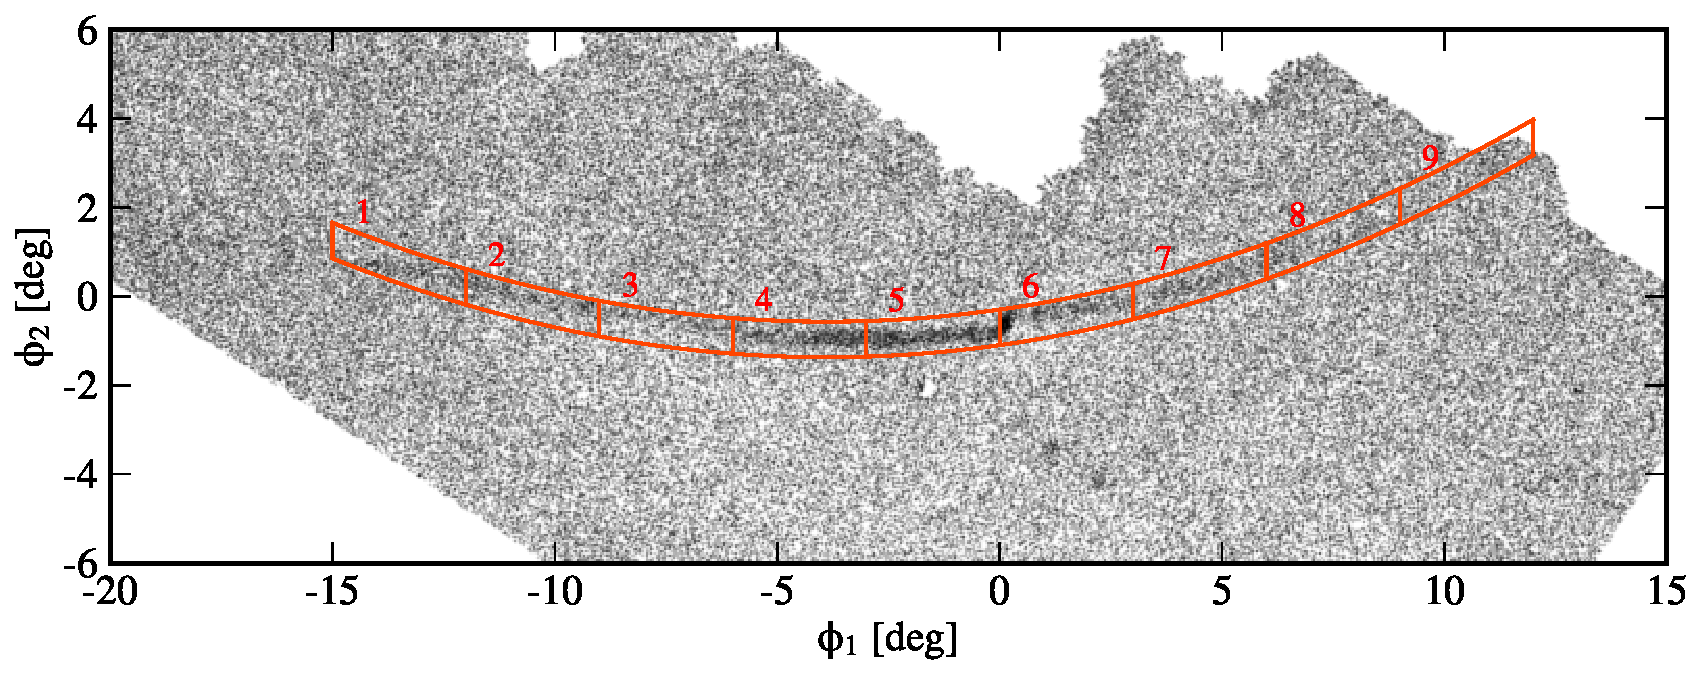
\includegraphics[width=0.85\textwidth]{fig1_a_map.pdf}
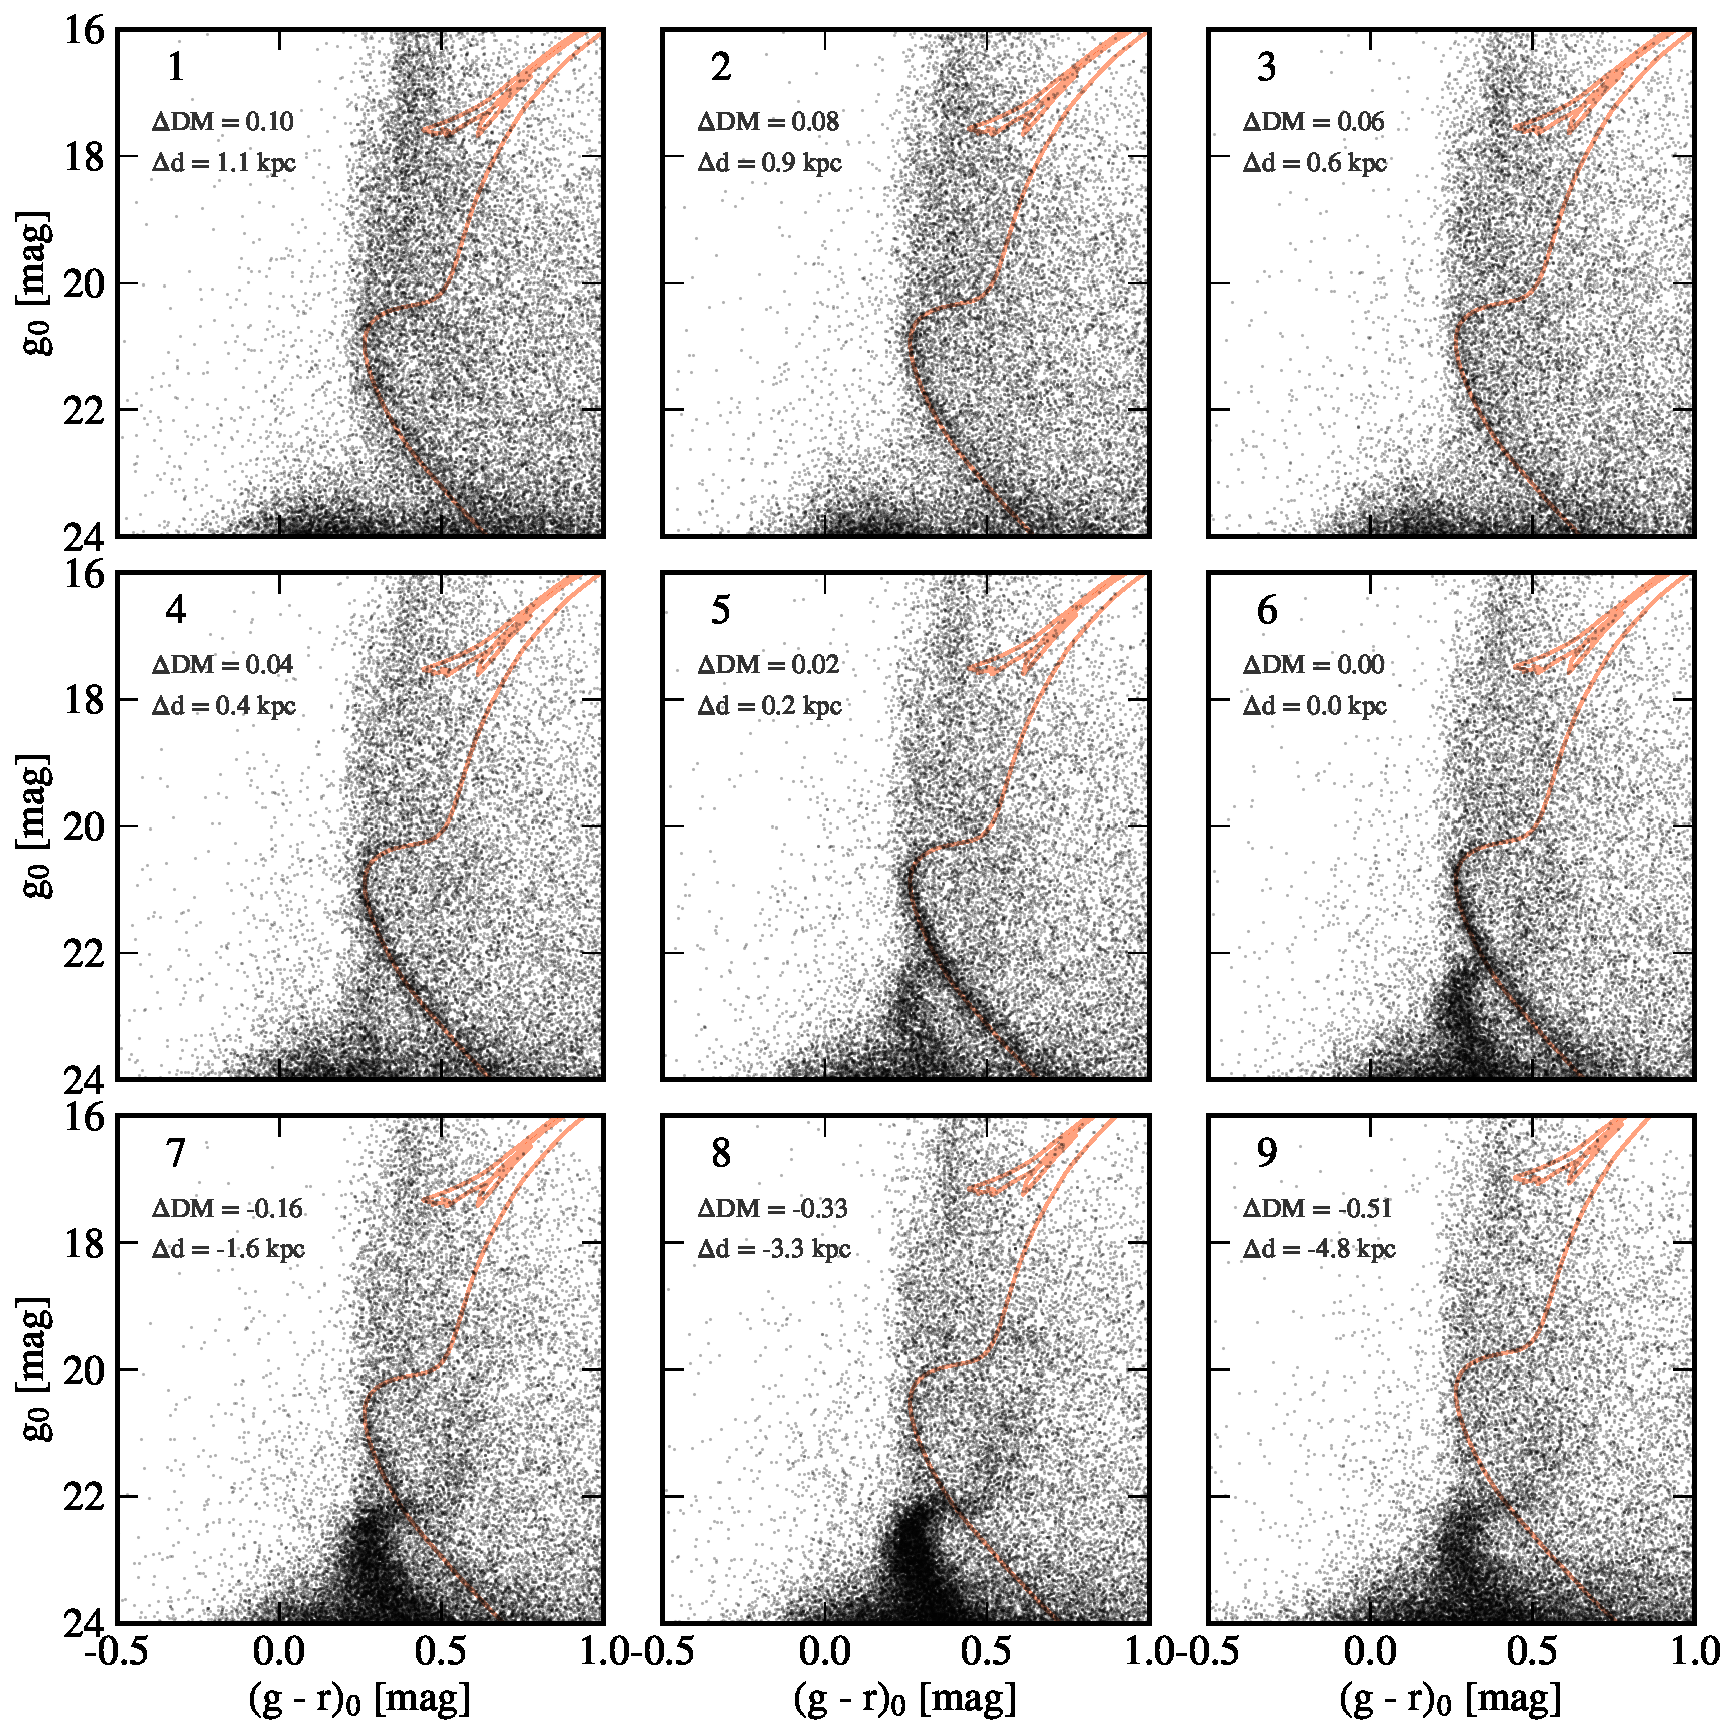
\includegraphics[width=0.85\textwidth]{fig1_b_cmds.pdf}
\end{center}
\caption{
(Top) The Legacy Surveys detection of the Palomar 5 globular cluster in a coordinate system aligned with its tidal tails.
(Bottom) Color-magnitude diagrams of $\approx0.8\times3$\,deg windows along the tails.
The regions are labeled in the top left of each panel, and their sky locations are marked in the top panel.
A stellar population consistent with Pal~5 is evident in every region, although its prominence varies between the fields.
There is a distance gradient along the stream, with the end of the trailing tail ($\phi_1\sim-15^\circ$) being the most distant, and end of the leading tail ($\phi_1\sim10^\circ$) the closest.
The fiducial Pal~5 isochrone is offset in every panel so that it matches the location of the main sequence, and the difference in distance modulus from the fiducial Pal~5 value is indicated in the top left.
}
\label{fig:cmds}
\end{figure*}

- to select likely pal5 stars, we query the database for point sources, satisfying these criteria:
- we removed stars with large parallaxes, but that's only a small fraction of the sample because the overlap between gaia and this deep data is small
- main selection in cmd, main sequence of an x Gyr isochrone with metallicity y
- selected stars shown in top panel of Figure~\ref{fig:cmds}, in pal5 coordinates (best-fitting great circle, cluster at 0,0, stream moving in positive phi1)
- to increase the contrast, we apply the isochrone selection at two distances: x kpc for $\phi_1<0$ and y kpc for $\phi_1>=0$
- for the first time, pal5 detected continuously between $-15^\circ$ and $7^\circ$ 

- to further tune our selection, we measure the distance gradient along the stream from the location of pal5's ms turnoff
- we analyze cmds in xdeg long and ydeg wide boxes following along the stream track (as illustrated in Figure~\ref{fig:cmds})
- individual cmds are shown in the bottom grid of Figure~\ref{fig:cmds}, overplotted with the isochrone at the adopted distance
- pal5 track, sgr kicking in in the leading tail
- pal5 ms evident in all, even field 9 where there is no obvious overdensity in the simply-selected stars
- indication of low surface-brightness features that may be recovered with these data

- cmds also show that galaxies start creeping in at faint magnitudes
- not surprising since only used structure, and faint galaxies are $\sim$ point sources
- in color-color space, stars and galaxies have different loci
- we select sources with:
- our z-band coverage is shallower, so to be somewhat homogeneous, we only select stars with $g<23.x$
- this still increases the contrast of pal5

\begin{figure*}
\begin{center}
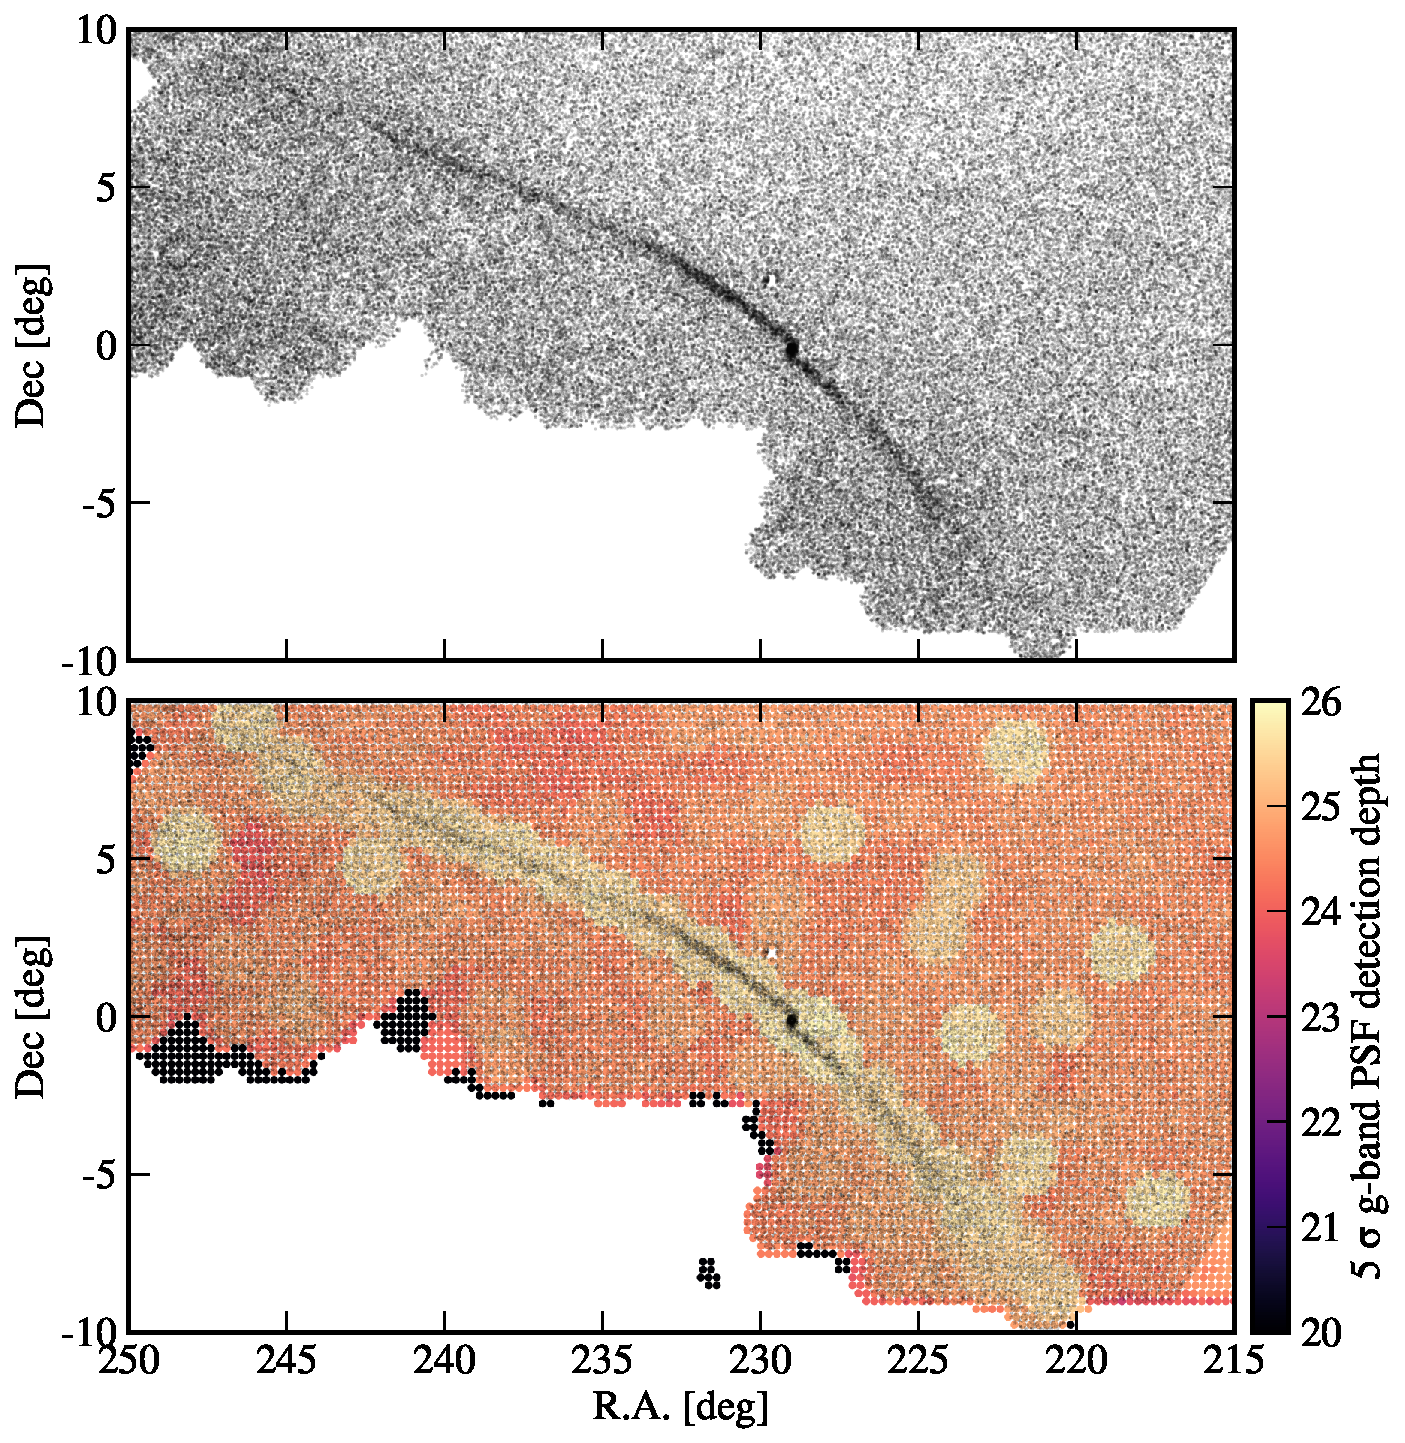
\includegraphics[width=0.85\textwidth]{fig2_maps.pdf}
\end{center}
\caption{
(Top) The optimized Legacy Surveys detection of the Palomar 5 system reveals an extremely wide, low surface-brightness extension of the leading tail beyond $\rm Dec<-5^\circ$.
Likely members are selected in the $g,\,g-r$ space as consistent with the Pal~5 main sequence (assuming the distance along the stream varies as mapped in Figure~\ref{fig:cmds}), with an additional selection on the stellar locus in the $g-r,\,g-z$ space.
(Bottom) Likely Pal~5 members overplotted on the map of $5\,\sigma$ PSF detection depth in the $g$-band (calculated in $0.5^\circ\times0.5^\circ$ bricks).
The Pal~5 region has been specifically targeted and is hence deeper than the nominal Legacy Surveys fields.
Some features in the distribution of likely Pal~5 members might be due to this variable depth, for example the asymmetry in the fan.
}
\label{fig:maps}
\end{figure*}

- Figure~\ref{fig:maps} shows the most likely members of Pal5
- these were selected to be stars in grz space, and on the Pal5 main sequence
- isochrone selection was done in xdeg bins of phi1, assuming the distance was constant in each bin, and equal to the interpolated value of the distance derived from the msto locations in Figure~\ref{fig:cmds}
- with these selections, pal5 stands high above the background between ra x and y

- the revised map of pal5 reveals qualitatively new features
- first, the leading tail extends past the previous footprint, and also appears to be widening
- next, the stellar density along the stream varies significantly
- previously detected gaps at ra, dec =(x,y) and (z,q) now made very prominent
- finally, the stream track is much better defined, and features sharp turns, e.g., at (ra,dec) = (x,y)
- we quantify these features in the next section

\section{Simulations}
\label{sec:sim}
To explore the mechanism leading the the observed morphology of the stream (i.e. the length asymmetry between the leading and trailing arm, as well as the gap in the trailing arm, and the ``fan" in the leading arm), we run a suite of Pal 5 simulations.
In particular, we investigate whether Pal 5's ``fan" in the leading arm can be explained due to chaotic regions in the potential (\citealt{Pearson:2015}, \citealt{Price-Whelan:2016}, Yavetz et al., {\it in prep.}), or whether Pal 5 is interacting with the Galactic bar (\citealt{Erkal:2017}, \citealt{Pearson:2017}, \citealt{Banik:2019}).
In Section \ref{sec:potential}, we describe the potentials we use to simulate the evolution of Pal 5, and in Section \ref{sec:modeling} we describe our simulation setup.
We show the results of our analyses in Section \ref{sec:sim_results}.

\subsection{Potential}
\label{sec:potential}
We simulate the evolution of Pal 5 in two classes of three-component Galactic potentials:

\begin{itemize}
\item[1.] {\bf Static potential}: we use the {\small MWPotential2014} (\citealt{Bovy:2015}) consisting of a Miyamoto-Nagai disk (\citealt{Miyamoto:1975}), a bulge modeled as an exponentially cut off, power-law density profile, and an NFW dark matter halo (\citealt{Navarro:1996}).
We vary the flattening of the NFW halo ($q_z = 0.94$ and $q_z = 0.5$) to investigate Pal 5's morphology on a regular as well as chaotic orbit (see Section \ref{sec:modeling}).

\item[2.] {\bf  Barred potential}: we use the same disk and halo as in the {\small MWPotential2014}, but include a Galactic bar instead of a bulge.
Following \citet{wang:2012}, we compute the bar potential as a basis-function expansion (BFE) representation of a triaxial, exponential density profile:

\begin{equation}
\rho_{bar} = \rho_0 [{\rm exp} (-r^2_1/2) + r_2^{-1.85} {\rm exp}(-r_2) ]
\end{equation}

\begin{equation}
r_1 = \left[\left((x/x_0)^2 + (y/y_0)^2\right)^2 +( z/z_0)^4\right]^{1/4}
\end{equation}

\begin{equation}
r_2 = \left[\frac{q^2(x^2 + y^2) + z^2)}{z_0^2}\right]^{1/2}
\end{equation}
where the scale lengths are $x_0$ = 1.49 kpc, $y_0$ = 0.58 kpc, $z_0$ = 0.4 kpc, and q = 0.6. We include terms up to $n=9$, $l=19$ in the ``self-consistent field" BFE formalism, as this yields a good representation of the density of the bar (\citealt{Banik:2019})\footnote{Note that using lower order terms (e.g. n=6, l = 8) for the basis function expansion does not much change the morphology or kinematics of the Pal 5 stream.}.
We explore barred models with pattern speeds of $\Omega_b$ = ($25 - 65$) $\kms$ kpc$^{-1}$ in increments of 1 kpc$^{-1}$, and  we test bar masses of $M_{bar} = 5 \times 10^{9}$ $\msun$ and $M_{bar} = 1 \times 10^{10}$ $\msun$ (\citealt{Portail:2017}).
Additionally, we fix the present day angular offset from the Galactic x-axis in the direction of rotation to $\alpha = 27\deg$.
\end{itemize}

\citet{wang:2012} constructed a bar with a pattern speed of $\Omega_b$ =  60 $\kms$ kpc$^{-1}$, which has a co-rotation radius, $r_{\rm CR} = 3.7$ kpc.
This is the radius at which the circular frequency ($\Omega_0$) is equal to the spin of the bar ($\Omega_b$) including the mass of the total potential.
In this paper, however, we explore a {\it range} of pattern speeds, which will lead to different co-rotation radii for different pattern speeds (faster bars have co-rotation at smaller radii and vice versa).
As bars are not expected to extend much beyond their co-rotation radius (\citealt{binney:2008}), we therefore adjust the physical scaling of the bar when we vary the pattern speed. %In \citet{wang:2012}, the scale-radius, $r_s$, assumed in the BFE, is  $r_s = 1.1$ kpc.

In particular, we  compute the co-rotation radius, $r_{\rm CR},$ for the mass profiles of the static potential for any given pattern speed, $\Omega_b$.
We then scale the bar model for a given pattern speed, $\Omega_b$, by:
\begin{equation}
r_{s, \Omega_b}  = r_{{\rm CR}, \Omega_b}/r_{{\rm CR, Wang 2012}}
\end{equation}
If this scaling is not included (as the case for bar models in e.g. %\citealt{price:2016b},
\citealt{Pearson:2017}, \citealt{Erkal:2017}, \citealt{Banik:2019}), this creates a too strong bar quadrupole for the faster pattern speeds, and a too weak bar quadrupole for the slower pattern speeds.

% In Figure \ref{fig:vcirc}, we show the circular velocity as a function of radius for the barred, three-component Galactic potential with $\Omega_b$ = ($25 - 65$) $\kms$ kpc$^{-1}$. The red lines correspond to the potentials with a bar mass of $M_{bar} = 5 \times 10^{9}$ $\msun$, and the blue lines correspond to potentials with a bar mass of  $M_{bar} = 1 \times 10^{10}$ $\msun$.
%
% \begin{figure}
% \centerline{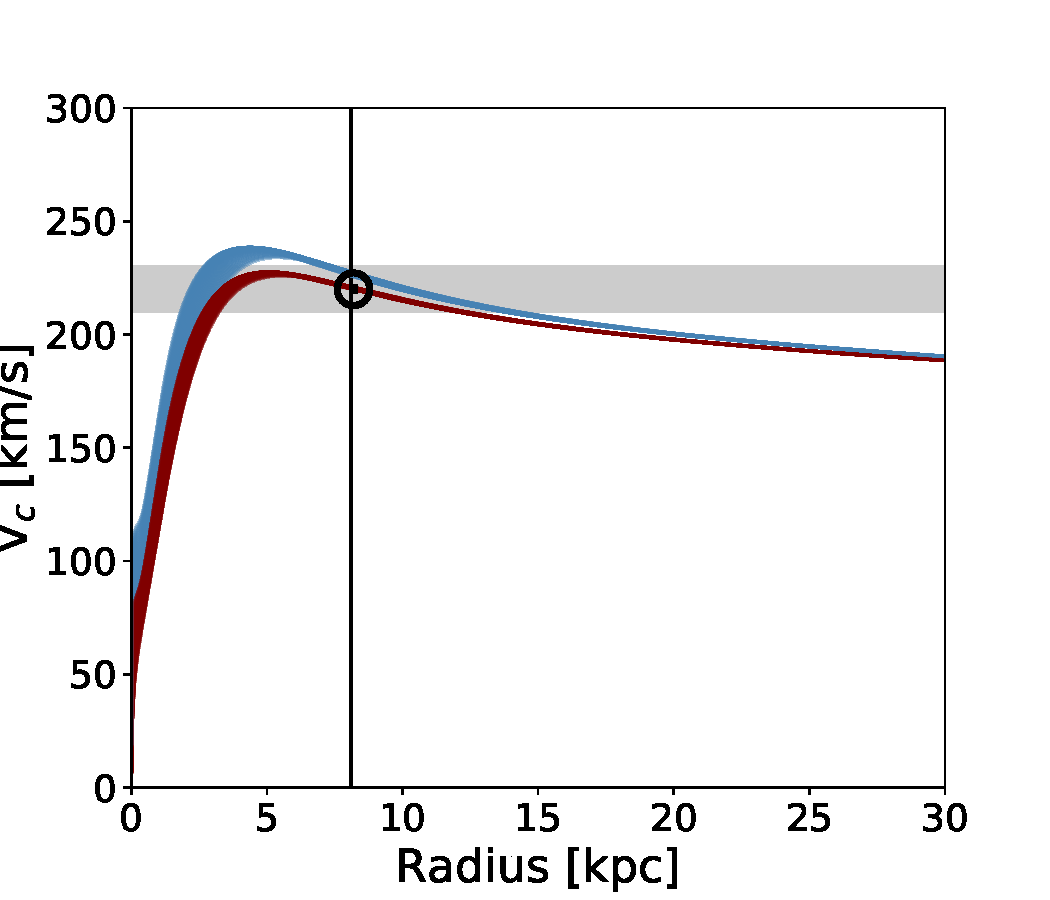
\includegraphics[width=\columnwidth]{v_circ_nlm919.pdf}}
% \caption{\todo{Probably include static potential as well, and show the different components of the potentials }}
% \label{fig:vcirc}
% \end{figure}


\subsection{Stream modeling}
\label{sec:modeling}
To simulate the evolution of Pal 5 in a given potential, we first transform Pal 5's observed 6D phase space coordinates into a Galactocentric frame by assuming $v_{lsr} = (11.1, 24.0, 7.25) ~\kms$,  $v_{circ} = 220  ~\kms$ and a distance from the Sun to the Galactic center of 8.1 kpc.
At the present, Palomar~5 globular cluster is at: RA = 229.018 deg, Dec = - 0.24 deg, distance = 22.9 kpc, $v_r$ = -58.7 , pm$_{RA,cosdec}= -2.296$ mas and pm$_{Dec} = -2.257$ mas.
We then integrate the cluster backwards in time for 4 Gyr in steps of 0.5 Myr in the potentials described in Section \ref{sec:potential}.
Subsequently, we simulate the forward evolution of Pal 5 using the ``particle-spray" stream generating method developed by \citet{Fardal:2015}, such that the cluster ends at its present day position at $t = 0$.
We release two particles through each of the two Lagrange points every 8 Myr.

To investigate Pal 5's evolution on a regular orbit, we first run a ``particle-spray" simulations setting $q_z = 0.94$ (\citealt{Bovy:2016}).
Subsequently, we run the same simulation setting $q_z = 0.5$ to induce a chaotic orbit.
Additionally, we simulate the evolution of Pal 5's stream in the barred potential, where we first integrating the orbit backwards for 4 Gyr, and then create mock streams as described above.
We vary the pattern speed of the bar, while updating its physical scaling (see Section \ref{sec:potential}. % and Figure \ref{fig:vcirc}).
We repeat this exercise using bar masses of both $M_{bar} = 5 \times 10^{9}$ $\msun$ and $M_{bar} = 1 \times 10^{10}$ $\msun$.

\subsection{Simulation results}
\label{sec:sim_results}
In Figure \ref{fig:sims}, we present the morphology (left column) and radial velocities (right column) of the simulated Pal 5 streams in various potentials.
The first two rows show Pal 5 evolved in a static potential with two different flattenings (see Section \ref{sec:potential}).
The last rows show four examples of Pal 5 evolved in barred potentials.
We selected these four examples through visual inspection of the density and width of the data and the simulated streams.

\begin{figure*}
% \centerline{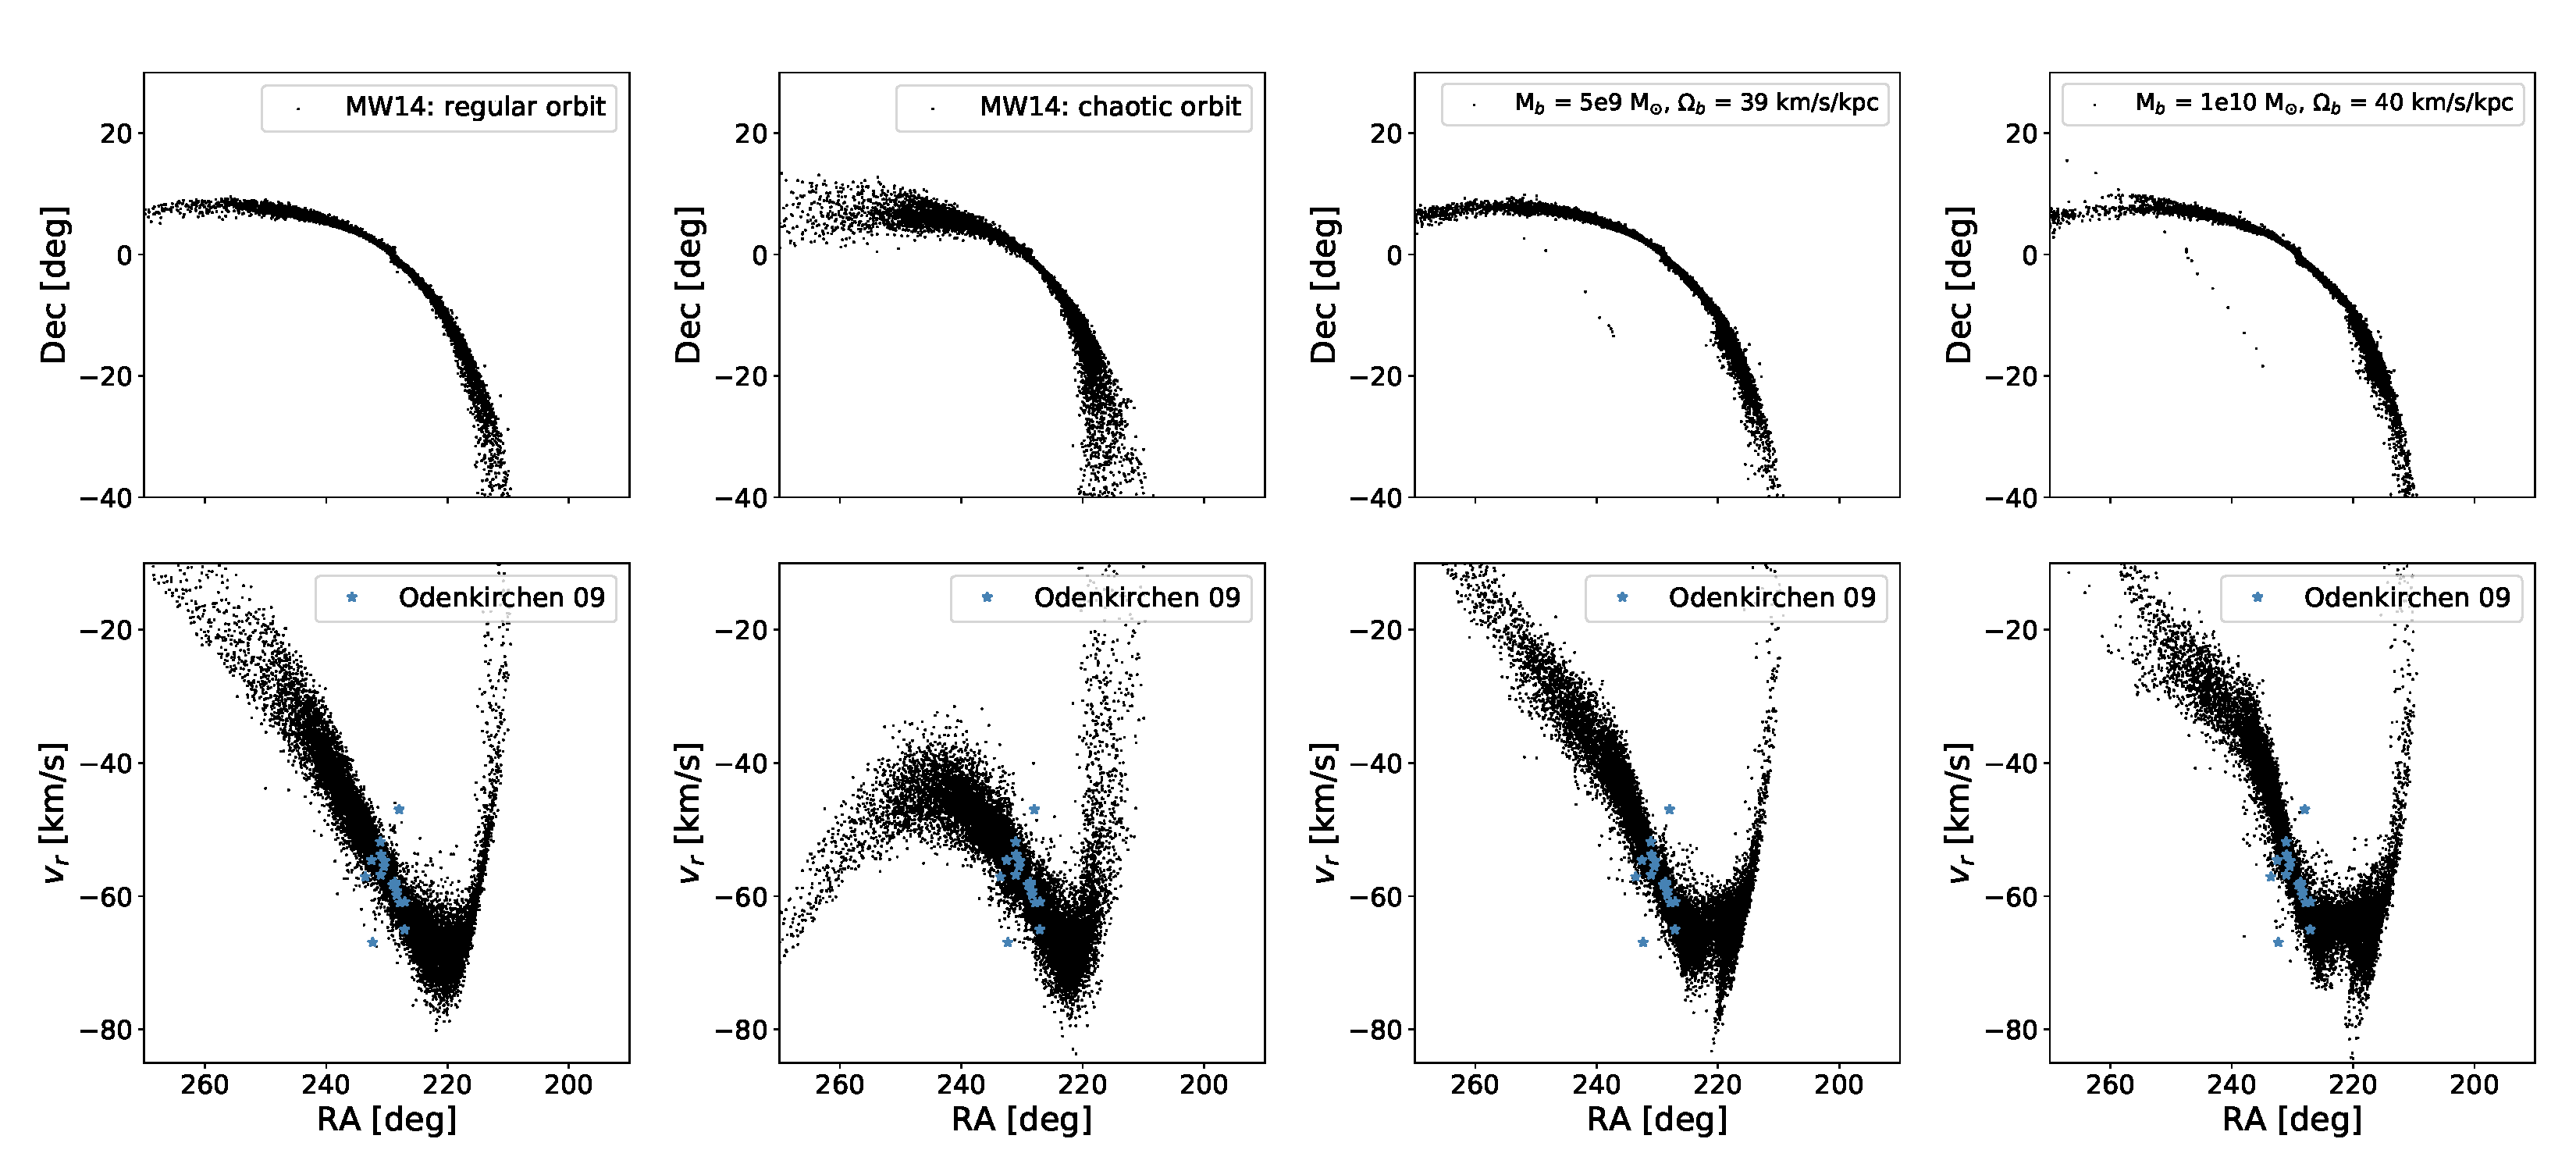
\includegraphics[width=\textwidth]{simulations.pdf}}
\caption{\todo{Something like the above, maybe with more bar models. Have separate plot in next section comparing the width and density of these to the width and density of the data using Gaussian mixture model. }}
\label{fig:sims}
\end{figure*}


% \section{Density model}
% \label{sec:density}
% To compare our data and various Pal 5 simulated streams, we construct density model consisting of a multicomponent Gaussian mixture model. In particular, we are interested in fitting the width and density of our data and simulated stars.
%
% We first transform our simulated Pal 5 data points to the tangent sky plane using a Zeanit (Lambert azimuthal) equal-area projection, such that we can define a Gaussian. We call these coordinates, $X$, $Y$.
%
% We then fit a 3rd order polynomial to the leading and trailing arm separately, in this projected space.
%
% We place K nodes, k, equally in distance along the polynomial fits to the leading and trailing arm.
%
% At each node, k, along the polynomial we find the tangent/parallel unit vector,  $\hat{u}$, and the perpendicular normal unit vector, $\hat{v}$, to the stream.
%
% At each node, k, we define the co-variance matrix, $\tilde{C_k}$:
%
% \begin{equation}
% \tilde{C_k} =
% \begin{pmatrix}
%     h^2 & 0  \\
%     0 & S_k^2  \\
% \end{pmatrix}
% \end{equation}
% where $h$ is bandwidth of the Gaussian components along the polynomial fit and $S_k$ is the  width of the Gaussians in the perpendicular (normal) direction of the stream at any node, k.
%
% We transform it from the space spanned by the $\hat{u}$,  $\hat{v}$ vectors to $X$, $Y$:
% \begin{equation}
% C_k = \rm{R} \tilde{C_k} \rm{R}^T
% \end{equation}
% where
% \begin{equation}
% \rm{R} =
% \begin{pmatrix}
%     \rm{cos} \theta & - \rm{sin} \theta  \\
%     \rm{sin} \theta & \rm{cos} \theta \\
% \end{pmatrix}
% \end{equation}
% and  $\theta$ is the angle between the tangent sky plane and the unit vector, $\hat{u}$.
%
% To compute our density model along the leading at trailing stream, for the K nodes, k, we define ln density  and sum over the K nodes:
% \begin{equation}
% \rm{ln} \sum ( \alpha_k \mathcal{N}\left(\mu_k, C_k\right))
% \end{equation}
% where $\mu_k$ denotes the location of each node, k, along the leading and trailing polynomial fits, respectively, $C_k$ is the covariance matrix, and $\alpha_k$ is the amplitude of the Gaussian (representing density at specific node, k).
%
% We then fit for the perpendicular width, $S_k$, to the stream (polynomial fits) and the amplitude of the Gaussians, $\alpha_k$, which represent the density along the stream.
%
% %Explain background model for data.
%
% We compute the width and density of both or simulated Pal 5 streams and the DECaLS data fitting the above Gaussian mixture model.




\section{Discussion}
\label{sec:discussion}

\subsection{Deeper stream data}
Do all streams look crazy if we get deeper data? Discuss ``stream-fanning", bar, VL2 Bonaca paper.

\subsection{Other perturbers}
As Pal 5 is moving prograde with respect to the disk it will be subject to interactions with both the bar (\citealt{Hattori:2016}%, \citealt{price:2016b}
), molecular clouds (\citealt{Amorisco:2016}) and possibly spiral arms (\citealt{Banik:2019}). Additionally, dark matter substructure could be interacting with the stream. Pal 5 apocentric distance is $\sim 18$ kpc, and the cluster is therefore probing the inner part of the Galatic potential. Hence, it might be unlikely that there are many dark matter subhalos in this part of the halo (\citealt{Garrison-Kimmel:2017}). However, the GD1 stellar stream orbit probes a similar region of the Galatic potential, and shows evidence of an interaction with a dark substructure (\citealt{Price-Whelan:2018}, \citealt{Bonaca:2018b}) as the data shows a gap and a ``spur" (\citealt{Yoon:2011}).



\section{Conclusion}
\label{sec:conclusion}


\acknowledgements{
It is a pleasure to thank


% \appendix
% \section{Math for density model}
% We define our likelihood function, $\mathcal{L} $, as:
%
% \begin{equation}
%     \begin{split}
%      \mathcal{L} = P(\{x_n\} \given \{\mu_k\}, \{C_k\}, \{\alpha_k\} ) &=
%             \prod_n \sum_k P(x_n \given \mu_k, C_k, \alpha_k )  \quad
%     \end{split}
% \end{equation}
% where $K$ is the total number of nodes, $\mu_k$ is the mean position of each node, $N$ is the total number of ``data points", $\alpha$ is the amplitude, $x_n$ = $\begin{pmatrix} x\\  y \end{pmatrix}$ is the data points and $P$ is:
% \begin{equation}
%     \begin{split}
%        P(x_n \given \mu_k, C_k, \alpha_k ) = \alpha_k \mathcal{N}(x_n \given \mu_k, C_k)  \quad
%     \end{split}
% \end{equation}
%
% $C_k$ is the covariance matrix in the $X,Y$-space which is the tangent plane sky projection. We transform to $X,Y$-space from the space spanned by the $\hat{u}$,  $\hat{v}$ vectors:
% \begin{equation}
% C_k^{(x,y)} = \rm{R} \tilde{C_k} \rm{R}^{\rm T}
% \end{equation}
% where
% \begin{equation}
% \tilde{C_k}^{(\hat{u},\hat{v})} =
% \begin{pmatrix}
%     {\rm h}^2 & 0  \\
%     0 & S_k^2  \\
% \end{pmatrix}
% \end{equation}
% and where h is bandwidth of the Gaussian components (which we fix) along the polynomial fit, and $S_k$ is the  width of the Gaussians in the perpendicular (normal) direction of the stream at any node, k. R is the rotation matrix from $\hat{u}$,  $\hat{v}$ to $X, Y$-space:
%
% \begin{equation}
% \rm{R} =
% \begin{pmatrix}
%     \rm{cos} \theta & - \rm{sin} \theta  \\
%     \rm{sin} \theta & \rm{cos} \theta \\
% \end{pmatrix}
% \end{equation}
% and  $\theta$ is the angle between the tangent sky plane and the unit vector, $\hat{u}$.
%
% To optimize for the likelihoods, we compute the analytic derivatives of the log likelihoods, ln$\mathcal{L}$:
%  \begin{equation}
%  \begin{split}
%     {\rm ln} \mathcal{L} = \sum_n {\rm ln} \left[\sum_k P(x_n \given \mu_k, C_k, \alpha_k)\right]  \quad
%     \end{split}
% \end{equation}
% hence, we want to compute:
%  \begin{equation}
%  \begin{split}
%     \frac{\partial{\rm ln} \mathcal{L}}{\partial \alpha_k}, \frac{\partial{\rm ln} \mathcal{L}}{\partial \mu_k}, \frac{\partial{\rm ln} \mathcal{L}}{\partial S_k}  \quad
%     \end{split}
% \end{equation}
%
% To do so, we need to use the following:
%  \begin{equation}
%  \begin{split}
%  |C_k^{-1}|^{1/2} = \frac{1}{{\rm h} S_k},
%    \end{split}
% \end{equation}
%
%  \begin{equation}
%  \begin{split}
%   \alpha_K = 1 - \sum_k^{K-1} \alpha_k,
%    \end{split}
% \end{equation}
%
%  \begin{equation}
%  \begin{split}
%  \mathcal{N}(x_n \given \mu_k, C_k) = \frac{1}{2\pi}|C_k^{-1}|^{1/2} {\rm exp}\left[-\frac{1}{2}(x_n - \mu_k)^{\rm T} C_k^{-1} (x_n - \mu_k) \right]  \quad
%    \end{split}
% \end{equation}
%
% We can now compute the partial derivatives of the log likelihoods, $\partial$ln$\mathcal{L}$:
%  \begin{equation}
%  \begin{split}
%     \frac{\partial{\rm ln} \mathcal{L}}{\partial \alpha_k}  = \sum_n \frac{ \mathcal{N}(x_n \given \mu_k, C_k) -  \mathcal{N}(x_n \given \mu_K, C_K)}{\sum_k \alpha_K \mathcal{N}(x_n \given \mu_K, C_K)} \quad
%     \end{split}
% \end{equation}
% \todo{check capital K's above}
% and
%
%  \begin{equation}
%  \begin{split}
% \frac{\partial{\rm ln} \mathcal{L}}{\partial \mu_k} = \sum_n \frac{\alpha_k \mathcal{N}(x_n \given \mu_k, C_k) C_k^{-1} (x_n - \mu_k)}{\sum_k \alpha_K \mathcal{N}(x_n \given \mu_K, C_K)}
%     \end{split}
% \end{equation}
% and
%
%  \begin{equation}
%  \begin{split}
% \frac{\partial{\rm ln} \mathcal{L}}{\partial S_k} = \sum_n \frac{\alpha_k \mathcal{N}(x_n \given \mu_k, C_k)}{\sum_k \alpha_K \mathcal{N}(x_n \given \mu_K, C_K)} \left[ \frac{1}{S_k} \left(\frac{1}{S_k^2} \left( \frac{1}{b_2} {\rm cos \theta} -  \frac{1}{b_1} {\rm sin} \theta \right)^2 - 1\right)\right]
%     \end{split}
% \end{equation}
% where
% $\begin{pmatrix} b_1\\  b_2 \end{pmatrix}= x_n - \mu_k$.
%
% %\begin{equation}
% %    \begin{split}
% %    p(\phi_2 \given \bs{\theta}) &=
% %            \alpha_{\textrm{bg}} \, \mathcal{U}(-10, 5) \\ & \quad +
% %            \alpha_{\textrm{s}, 1} \, \mathcal{N}(\phi_2 \given \mu_{\textrm{s}}, \sigma_{\textrm{s}, 1}) +
% %            \alpha_{\textrm{s}, 2} \, \mathcal{N}(\phi_2 \given \mu_{\textrm{s}}, \sigma_{\textrm{s}, 2}) \\ & \quad +
% %            \alpha_{\textrm{f}} \,
% %                \mathcal{N}(\phi_2 \given \mu_{\textrm{f}}, \sigma_{\textrm{f}})
% %    \end{split}
% %\end{equation}
%
%
% %
% % This work has made use of data from the European Space Agency (ESA) mission {\it
% % Gaia} (\url{https://www.cosmos.esa.int/gaia}), processed by the {\it Gaia} Data
% % Processing and Analysis Consortium (DPAC,
% % \url{https://www.cosmos.esa.int/web/gaia/dpac/consortium}). Funding for the DPAC
% % has been provided by national institutions, in particular the institutions
% % participating in the {\it Gaia} Multilateral Agreement.  This research was
% % started at the NYC Gaia DR2 Workshop at the Center for Computational
% % Astrophysics of the Flatiron Institute in 2018 April.
% %
% % AB acknowledges generous support from the Institute for Theory and Computation
% % at Harvard University.
% % All code used in this work and all results are available at
% % \url{https://github.com/adrn/GD1-DR2}.
% }

\software{
    \package{Astropy} \citep{astropy, astropy:2018},
    \package{dustmaps}\footnote{\url{https://github.com/gregreen/dustmaps}},
    \package{gala} \citep{gala},
    \package{IPython} \citep{ipython},
    \package{matplotlib} \citep{mpl},
    \package{numpy} \citep{numpy},
    \package{scipy} \citep{scipy}
}

\bibliographystyle{aasjournal}
\bibliography{pal5fan}

\end{document}
